\section{Durchführung/Aufbau}
\label{sec.Durchführung}

   \subsection{Bestimmung des Eigenträgheitsmoments und der Winkelrichtgröße}

   Zu Beginn wird eine massenlose Stange,
   die zuvor gewogen und ausgemessen wurde,
   auf der Apperatur festgeschraubt.
   Die Apperatur ist in Abbildung \ref{fig:1} zu sehen.
   Die Stange wird nun um zehn unterschiedliche Winkel $\varphi$ ausgelenkt.
   Zu jedem Winkel wird die wirkende Kraft mit einem Federkraftmesser bestimmt.
   \\
   Im Anschluss werden zwei Gewichte, die als symmetrisch angenommen werden,
   ausgemessen und gewogen.
   An der Stange befinden sich diese Gewichte jeweils zum selben Abstand von der Drehachse.
   Sie werden per Hand um einen bestimmten Winkel $\varphi$ ausgelenkt und losgelassen.
   Die Periodendauer $T$ der entstandenen Schwingung wird mittels einer Stopuhr bestimmt.
   Dies wird für zehn unterschiedliche Abstände von der Drehachse durchgeführt.

   \begin{figure}
    \centering
    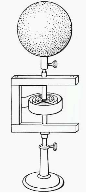
\includegraphics[scale=0.8]{V101_Aufbau.png}
    \caption{Aufbau der Apperatur am Beispiel einer Kugel}
    \label{fig:1}
   \end{figure}

   \subsection{Das Trägheitsmoment zwei unterschiedlicher Körper}

      Nun wird der Stab durch einen Zylinder ausgetauscht.
      Auch dieser wird zuvor gewogen und ausgemessen.
      Der Körper besitzt eine Makierung, die als Nullpunkt verwendet wird
      um den Körper um einen
      gleichbleibenden Winkel $\varphi$ auszulenken.
      Es wird wieder die Periodendauer $T$ mittels einer Stoppuhr bestimmt.
      Der Vorgang wird fünfmal wiederholt und
      anschließend mit einer Kugel durchgeführt.

   \subsection{Trägheitsmoment einer Puppe}

      Die in 3.2 beschriebene Messung wird für eine Holzpuppe ebenfalls wiederhohlt.
      Dafür wird die Puppe gewogen und ausgemessen.
      Für die Ausmessung werden die Arme, der Rumpf, die Beine und der Kopf
      jeweils als Zylinder genährt.
      Die Breite jedes Körperteils ist fünf mal zu messen um einen Mittelwert
      des Radius für den Zylinder zu erhalten.
      Die Periodendauer $T$ wird für eine stehende Puppe mit ausgestreckten Armen bestimmt.
      Anschließend für diese Puppe in sitzender Position mit ausgestreckten Armen.
